\documentclass{beamer}
\usepackage[utf8]{inputenc}
\usepackage{verbatim}
\usepackage{tikz}
\usetheme{Madrid}
\usetikzlibrary{patterns}
\usetikzlibrary{shapes.geometric}
\title[Tic]{CSE 300 Online on Tikz and Beamer}
\author{1605042}
\date{\today}
\tikzstyle{myBox} = [trapezium,trapezium left angle=60,trapezium right angle=120]
\begin{document}
	\maketitle
	\begin{frame}
		\frametitle{Table of Contents}
		\tableofcontents
	\end{frame}
	\section{Introduction}
	\begin{frame}
		Beamer is more useful than powerpoint for many reasons:
		\begin{itemize}
			 \item<1-> Consistent typesetting everywhere
			 \item<1-> Easy math and equations
			 \item<2-> Easy plotting of graphs
		\end{itemize}
	\end{frame}
	\section{An Example of Literature Review}
	\begin{frame}{Literature Review Sample}
	Summary of the relevant papers can be shown in presentation in elegant
	way using \LaTeX. Here is an example
	\begin{block}{Soliman, Hikal, Sakr; 2012}
		A comparative performance evaluation of intrusion detection techniques
		for hierarchical wireless sensor networks
	\end{block}
	
	\begin{columns}
		\column{0.5\textwidth}
		\begin{itemize}
		\item This paper evaluates and
		compares the most prominent
		anomaly-based IDS systems for
		hierarchical WSNs and
		identifying their strengths and
		weaknesses.
		\end{itemize}
		\column{0.5\textwidth}
		\begin{itemize}
			\item For each IDS, the architecture
			and the related functionality are
			briefly introduced, discussed,
			and compared, focusing on both
			the operational strengths and
			weakness.
		\end{itemize}
	\end{columns}
	\end{frame}
	\section{Flowchart}
	\begin{frame}{A Flowchart}
		Flowchart of finding whether an input number is even or odd is shown:
		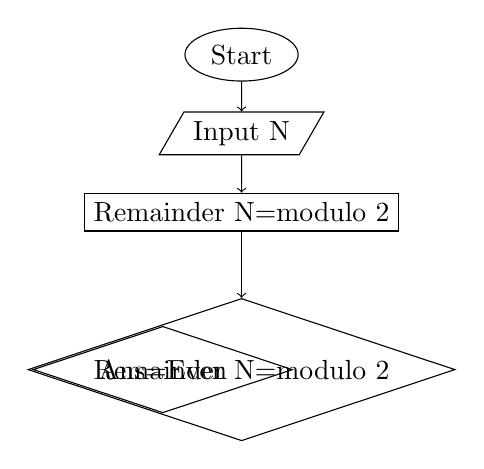
\begin{tikzpicture}[align=center]
			\node[draw,ellipse,aspect=3,align=center, xshift=5cm, yshift=-3cm] (n1) at (10,0) {Start};
			\node[draw,myBox,below of=n1] (n2) {Input N};
			\node[draw,rectangle,below of=n2] (n3) {Remainder N=modulo 2};
			\node[draw,diamond,below of=n3,aspect=3,yshift=-1cm] (n4) {Remainder N=modulo 2};
			\draw[->] (n1.south)--(n2.north);
			\draw[->] (n2.south)--(n3.north);
			\draw[->] (n3.south)--(n4.north);
			\node[draw,diamond,left of=n4,aspect=3] (n5) {Ans=Even};
			
			
		\end{tikzpicture}
	\end{frame}
	
\end{document}